\documentclass[11pt,a4paper]{article}

\usepackage[utf8]{inputenc}
\usepackage[T1]{fontenc}
\usepackage{geometry}
\geometry{margin=2.5cm}
\usepackage{parskip}
\usepackage{xcolor}
\usepackage{listings}
\usepackage{hyperref}
\usepackage{titlesec}
\usepackage{graphicx}

\title{\textbf{FSStat - Report}}
\author{Martin Tomassi}
\date{}

\begin{document}
\maketitle

\section{Problem Analysis}

This assignment involves designing a library that exposes an asynchronous operation capable of calculating size-based statistics on a directory tree: the total number of files contained in a directory (including all of its subdirectories recursively), along with a histogram of file sizes distributed across equally spaced bands ranging from 0 to the maximum file size, plus an overflow band that includes files larger than the maximum file size. From a concurrent point of view, this problem naturally lends itself to a fork/join-style tree traversal. The directory hierarchy has a structure and depth that are unknown a priori, so the traversal strategy must recursively generate independent subtasks for each subdirectory encountered and subsequently reconcile their partial results into a single coherent \texttt{FSReport}. Two aspects make the problem non-trivial when a concurrent solution is required:

\begin{itemize}
	\item \textbf{I/O-bound workload.} Listing directory entries and reading file metadata are system calls that block the calling thread while the underlying operation completes. A purely sequential, single-threaded traversal would leave the CPU idle for most of the execution time, since the bottleneck is disk/OS latency rather than computation.
	\item \textbf{Result aggregation under concurrency.} Because sub-directories are explored independently and potentially in parallel, the partial results produced by different branches of the tree must eventually be merged into one coherent \texttt{FSReport}. This merge must be free of race conditions and must not lose or double-count any file, regardless of the order or degree of parallelism with which the various branches complete.
\end{itemize}

Since directory entries belonging to the same parent are read once and then dispatched to independent tasks, there is no shared mutable state accessed concurrently by unrelated branches of the traversal, other than the final aggregation step. Consequently, synchronization is not required to enforce mutual exclusion over shared mutable state, but rather to achieve task coordination: determining when every sub-task spawned for a directory has completed so that its results can be safely combined with those of its parent. No cyclic wait conditions arise because the directory tree is acyclic and traversal only ever waits on its own children, so deadlock is not a structural risk in any of the adopted approaches.

\section{Implementation Strategy}

The three variants are intentionally kept independent, allowing each implementation to fully exploit the strengths of its underlying concurrency model. Architecturally, they follow two different result-delivery models:

\begin{itemize}
	\item \textbf{One-shot aggregation (Event loop and Virtual Threads):} These implementations are designed for batch-oriented execution. Intermediate progress remains internal, and a single aggregated \texttt{FSReport} is returned once the scan completes.
	\item \textbf{Continuous event streaming (Reactive programming):} The RxJava implementation is designed for interactive GUI applications. Its push-based execution model naturally represents continuously evolving computation, enabling incremental progress updates, cancellation, and resource management while minimizing explicit thread coordination in the application logic.
\end{itemize}

\subsection{Event loop implementation (Vert.x)}

The Event loop implementation runs the entire traversal on a single Vert.x instance, using its non-blocking file-system API and a Future-based Continuation-Passing Style (CPS). Requests to list directory entries (\texttt{readDir}) and fetch file properties (\texttt{props}) are non-blocking from the perspective of the Event loop thread, as Vert.x delegates the underlying OS system calls to its internal worker thread pool. Traversal logic is expressed through asynchronous recursion between directory scanning (\texttt{scanDirectory}) and entry evaluation (\texttt{processFSEntry}), composed via \texttt{Future.compose} continuations rather than traditional synchronous call-stack recursion. In this way, the Event loop thread never blocks while I/O operations are in progress and remains continuously available to handle other events. Recursion over directory entries produces a list of child futures (\texttt{List<Future<FSReport>>}). Subdirectories trigger a recursive directory scan, whereas regular files immediately produce a single completed \texttt{FSReport}. These child futures are joined without blocking by waiting on the entire collection at once using composite futures (\texttt{Future.all}). Once all subtrees in a directory resolve, a \texttt{map} transformation merges the list of child reports into a single aggregated \texttt{FSReport}.

\subsection{Virtual threads implementation}

Execution is managed by an \texttt{ExecutorService} (\texttt{Executors.newVirtualThreadPerTaskExecutor()}), spawning a dedicated virtual thread task for each directory subtree encountered. Concurrency explicitly mirrors the file-system tree through a divide-and-conquer pattern: forking occurs when a subdirectory is discovered and submitted to the executor as a new task, while joining takes place when the parent task sequentially awaits child results via \texttt{childFuture.get()} before aggregating them. Within a single task, directory listing and attribute fetching are performed using traditional blocking Java NIO APIs (\texttt{Files.newDirectoryStream} and \texttt{Files.readAttributes}). Sizes of discovered regular files are accumulated locally within a task-confined \texttt{FSReportAccumulator} instance. Whenever a virtual thread performs a blocking operation, whether waiting on file-system I/O or on a child task's completion,the JVM transparently unmounts the virtual thread from its carrier thread, freeing OS thread resources to process other tasks. Once the blocking operation completes, the virtual thread is remounted onto an available carrier thread to resume execution. After processing local directory entries, the task converts its accumulator into an initial \texttt{FSReport} and iterates through the list of child futures, merging their sub-reports via \texttt{result.merge(childFuture.get())}.

\subsection{Reactive programming implementation (RxJava) and GUI extension}

Designing the library around RxJava provided several key architectural advantages for both the core API and its Swing extension. Rather than forcing the UI to poll or rely on shared mutable state, the reactive pipeline emits a stream of progressively updated \texttt{FSReport} snapshots, culminating in the final aggregated report. The library encapsulates blocking file-system calls within \texttt{Flowable.fromCallable} and delegates execution to a dedicated thread pool via \texttt{subscribeOn(Schedulers.io())}. Directory handles are managed using the \texttt{Flowable.using} pattern, ensuring deterministic cleanup of operating system file descriptors (\texttt{DirectoryStream::close}) upon completion, error, or early cancellation. As file sizes are emitted, they are mapped into unit \texttt{FSReport} instances and progressively folded into a running cumulative \texttt{FSReport} via a reactive \texttt{scan} operation. To serve both live UI updates and the final report without duplicating the traversal, the stream is multicasted using \texttt{publish}: one branch applies rate-limiting via \texttt{sample(100, TimeUnit.MILLISECONDS, Schedulers.computation())} to protect the Event Dispatch Thread (EDT) from high-frequency event floods, while a parallel branch uses \texttt{takeLast(1)} to capture the final aggregated report. These branches are merged via \texttt{Flowable.merge} and filtered with \texttt{distinctUntilChanged()} to suppress duplicate emissions. A Swing GUI connects directly to this reactive stream, marshalling incoming report snapshots onto the EDT to update live counters and the panel displaying the size distribution histogram. Scanning can be stopped at any time by disposing of the active \texttt{Disposable} subscription, which propagates cancellation upstream and triggers immediate resource cleanup. To prevent race conditions when scans are rapidly restarted, a monotonically increasing token is used to discard stale updates belonging to cancelled scans.

\begin{figure}[h]
	\centering
	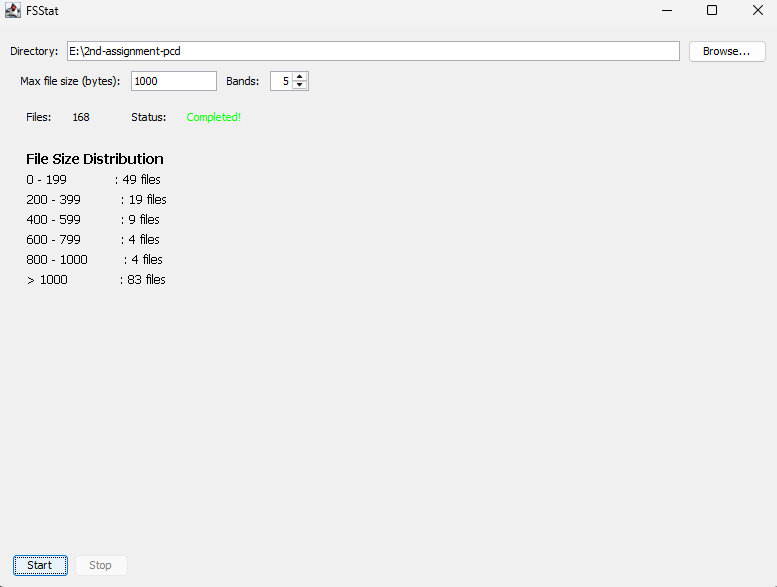
\includegraphics[width=\textwidth]{images/gui.png}
	\caption{Swing GUI built on top of the reactive implementation.}
	\label{fig:gui}
\end{figure}

\end{document}
